\documentclass{article}
\usepackage[utf8]{inputenc}
\usepackage{hyperref}
\usepackage[letterpaper, portrait, margin=1in]{geometry}
\usepackage{enumitem}
\usepackage{amsmath}
\usepackage{booktabs}
\usepackage{graphicx}

\usepackage{titlesec}

\titleformat{\section}
{\normalfont\Large\bfseries}{\thesection}{1em}{}[{\titlerule[0.8pt]}]
  
\title{Homework 3 Answers}
\author{Economics 7103}
\date{}
  
\begin{document}
  
\maketitle

\noindent 1. The Cobb-Douglas functional form is commonly assumed because of its flexibility and the ability of the researcher to estimate its parameters after taking logs.
\begin{enumerate}[label=(\alph*)]
    \item Simply use the rules of logarithms:
    \begin{align}
        y_i &= e^{\alpha} \delta^{d_i} z_i^{\gamma}  e^{\eta_i} \\
        ln(y_i) &= ln\left( e^{\alpha} \delta^{d_i} z_i^{\gamma}  e^{\eta_i} \right) \\
        & = ln\left( e^{\alpha} \right) + ln\left( \delta^{d_i} \right) + ln\left( z_i^\gamma \right) + ln\left( e^{\gamma_i} \right) \\
        & = \alpha ln(e) + ln(\delta)d_i + \gamma ln(z_i) + \eta_i ln(e) \\
        & = \alpha + ln(\delta) d_i + \gamma ln(z_i) + \eta_i.
    \end{align}
    \item $\delta$ is the energy efficiency multiplier induced by the retrofit program.  When $d_i = 0$ and there is no treatment, the $\delta$ term drops out of the energy use function.  When $d_i = 0$ and there is treatment, $\delta$ multiplicatively affects energy use.  If $\delta < 1$, then home energy efficiency increases due to the program.
    \item Simply perform algebraic manipulation to take the discrete version of the first derivative with respect to $d_i$:
    \begin{align}
        \frac{\Delta y_i}{\Delta d_i} & = y_i(d_i = 1) - y_i(d_i = 0) \\
        & = e^{\alpha} \delta z_i^{\gamma}  e^{\eta_i} - e^{\alpha} z_i^{\gamma}  e^{\eta_i} \\
        & = (\delta - 1) e^{\alpha} z_i^{\gamma}  e^{\eta_i}.
    \end{align}
    Multiply by $1 = \frac{y_i}{y_i}$:
    \begin{align}
        & = (\delta - 1) e^{\alpha} z_i^{\gamma}  e^{\eta_i} \frac{y_i}{e^{\alpha} \delta^{d_i} z_i^{\gamma}  e^{\eta_i}} \\
        & = \frac{\delta - 1}{\delta^{d_i}} y_i.
    \end{align}
    Intuitively, this is the amount of electricity saved by the retrofit program in KwH.
    \item It's easier to start with $ln(y_i)$. Exponentiate and take the partial derivative and perform algebraic manipulation to get the result:
    \begin{align}
        ln(y_i) &= \alpha + ln(\delta) d_i + \gamma ln(z_i) + \eta_i \\
        y_i &= exp\left( \alpha + ln(\delta) d_i + \gamma ln(z_i) + \eta_i \right) \\
        \frac{\partial y_i}{\partial z_i} &= \frac{\gamma}{z_i} exp\left( \alpha + ln(\delta) d_i + \gamma ln(z_i) + \eta_i \right).
    \end{align}
    Notice that $y_i = exp\left( \alpha + ln(\delta) d_i + \gamma ln(z_i) + \eta_i \right)$ and substitute this in to see:
    \begin{align}
        &= \gamma \frac{y_i}{z_i}.
    \end{align}
    $\frac{\partial y_i}{\partial z_i}$ is the change in $y_i$ for a change in $z_i$, holding all else equal; thus, it is the change in electricity used in home $i$ for a change square feet holding all else equal.
    \item Confidence intervals are more intuitive than standard errors, though one must always recall their interpretation: a 95-percent confidence interval states that if you were to independently sample from the population and perform this estimation over and over again, the estimate of the parameter will fall within the confidence interval 95 percent of the time.  See table \ref{tab:outputtable4} for the regression output.
    \begin{table}[h]
        \centering
        \begin{tabular}{lll}
\toprule
 & Coefficients & Marginal effects (dy/dx) \\
\midrule
retrofit & -0.10 & -113.98 \\
  & (-0.11, -0.09) & (-127.93, -99.21) \\
ln(sqft) & 0.89 & 0.63 \\
  & (0.88, 0.91) & (0.62, 0.64) \\
ln(temp) & 0.28 & 4.00 \\
  & (0.05, 0.53) & (0.72, 7.47) \\
Constant & -0.77 &   \\
  & (-1.85, 0.26) &   \\
Observations & 1000.00 & 1000.00 \\
\bottomrule
\end{tabular}

        \caption{Regression estimates for the log-log regression with calculated marginal effects.  95 \% confidence intervals bootstrapped using 1,000 replications.}
        \label{tab:outputtable4}
    \end{table}
    \item See figure \ref{fig:mfx}.
    \end{enumerate}
\begin{figure}[h]
    \centering
    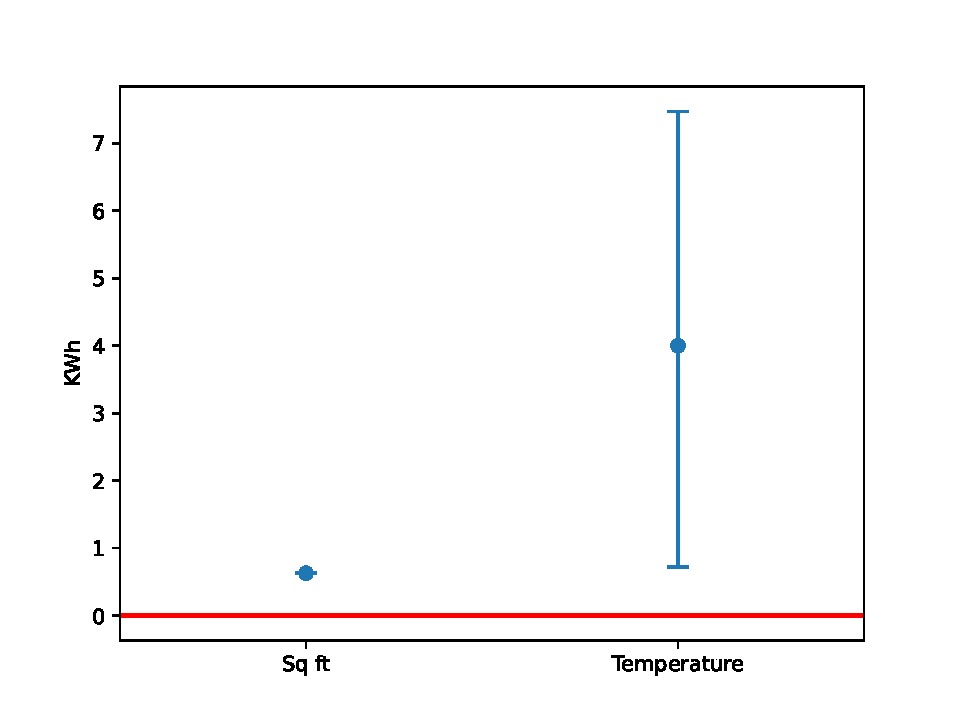
\includegraphics[scale=0.7]{mfx.pdf}
    \caption{Marginal effects with bootstrapped 95\% confidence intervals from the log-log regression.  Note that there is a confidence interval for the effect of an additional degree, but the parameter is estimated very precisely.}
    \label{fig:mfx}
\end{figure}

\end{document}